\section{Gestión del Proyecto en Jira}

Para la planificación y seguimiento del desarrollo del proyecto se ha utilizado la herramienta \textbf{Jira}. En esta plataforma se han recogido y priorizado todas las Historias de Usuario (HU), así como la asignación de sus correspondientes tareas y criterios de aceptación para la primera iteración.

\subsection{Configuración del Espacio y Priorización}
En el tablero del espacio \textbf{Doble M}, se organizan las HU estableciendo su orden y prioridad de ejecución. Para configurar los campos requeridos en el tipo de actividad \textit{Story}, se han seguido los siguientes pasos en la plataforma:
\begin{enumerate}
    \item Navegar a \textbf{Jira} $\rightarrow$ seleccionar el espacio \textbf{Doble M}.
    \item Hacer clic en el menú de opciones (\textbf{\dots}) $\rightarrow$ \textbf{Configuración del espacio}.
    \item Acceder al apartado \textbf{Tipos de actividad} y seleccionar \textbf{Story}.
    \item Cumplimentar los campos obligatorios y personalizados definidos para las historias de usuario.
\end{enumerate}

\begin{figure}[htbp]
    \centering
    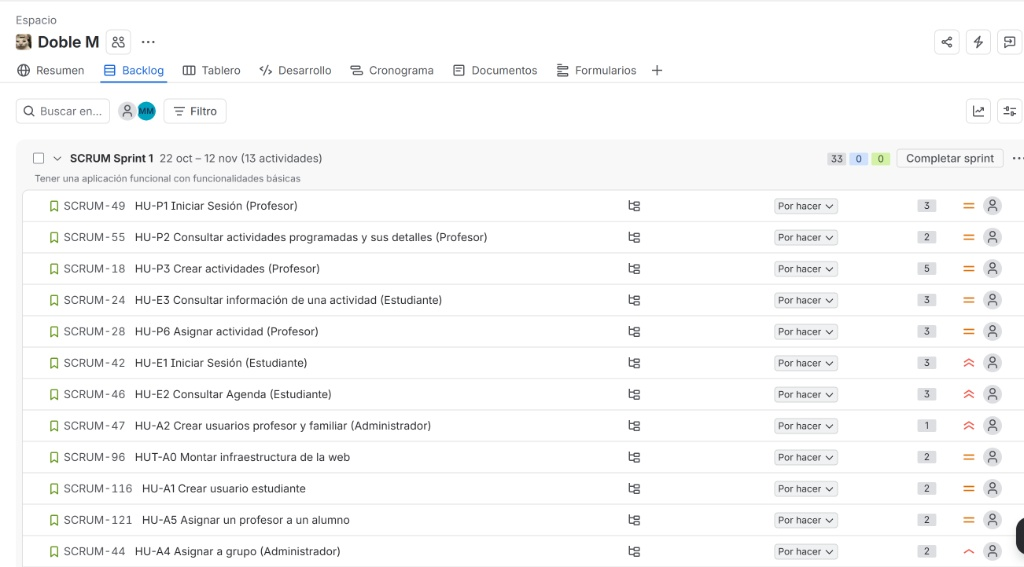
\includegraphics[width=0.95\textwidth]{img/jira_backlog.png}
    \caption{Vista general del Backlog en Jira con las Historias de Usuario priorizadas.}
    \label{fig:jira_backlog}
\end{figure}

\begin{figure}[htbp]
    \centering
    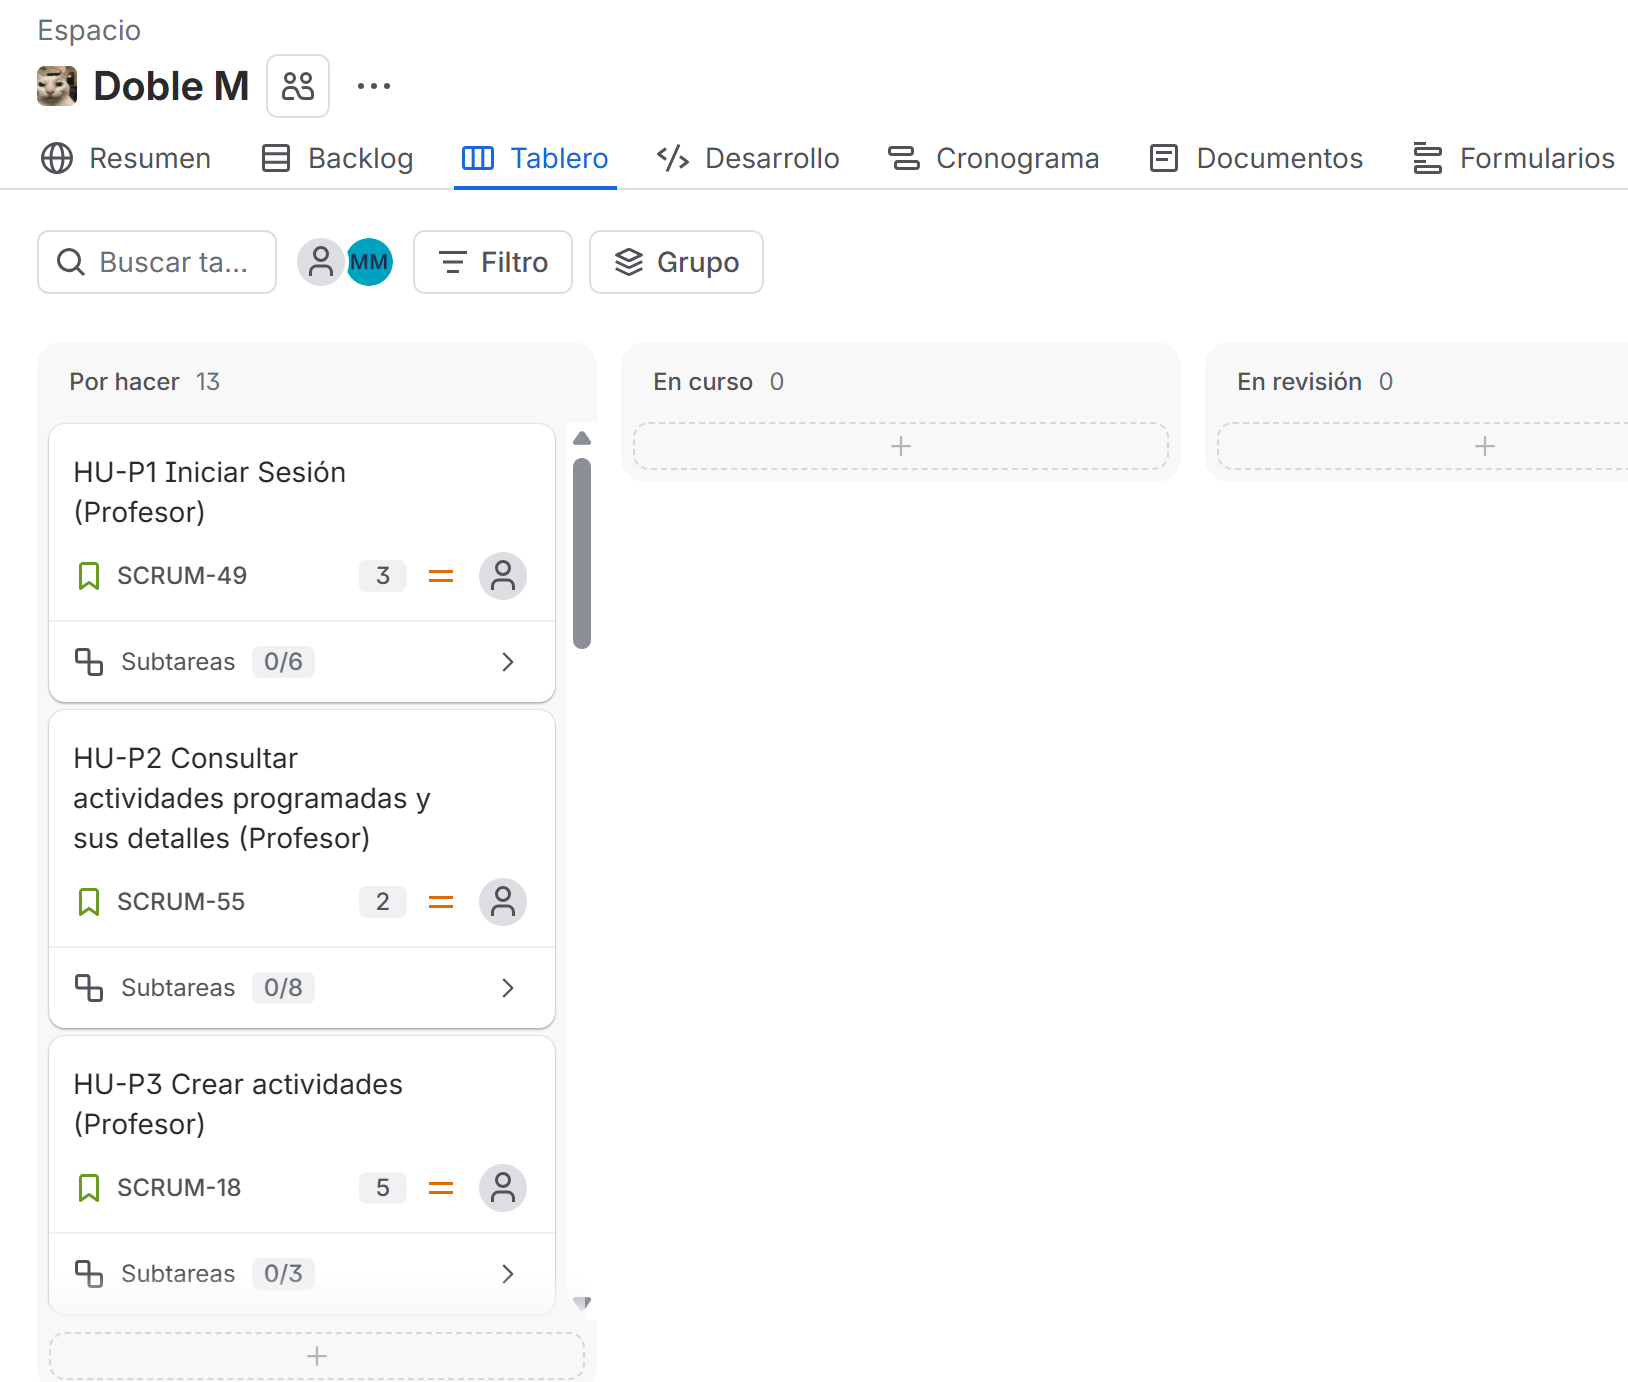
\includegraphics[width=0.95\textwidth]{img/jira_tablero.png}
    \caption{Vista del Tablero de Jira con las subtareas desplegadas.}
    \label{fig:jira_tablero}
\end{figure}